%
% Monografia de TCC1 de Douglas Brauner
%
\documentclass[twoside,english,brazilian]{UNISINOSmonografia}
\usepackage[utf8]{inputenc} % charset do texto (utf8, latin1, etc.)
\usepackage[T1]{fontenc} % encoding da fonte (afeta a sep. de sílabas)
\usepackage{graphicx} % comandos para gráficos e inclusão de figuras
\usepackage{bibentry} % para inserir refs. bib. no meio do texto
\usepackage{tabularx}
%=======================================================================
\unisinosbst

%=======================================================================
% Dados gerais sobre o trabalho.
%=======================================================================
\autor{Brauner}{Douglas}
\titulo{Elasticidade Baseada em Containers para Aplicação de Alto Desempenho}
%\subtitulo{sub}
\orientador[Prof.~Dr.]{Righi}{Rodrigo da Rosa}
%\coorientador[Prof.~Dr.]{Lamport}{Leslie}
\local{São Leopoldo}
\ano{2016}

\unidade{Unidade Acadêmica Graduação}
\curso{Curso de Bacharelado em Ciência da Computação}
\natureza{%
Trabalho de Conclusão de Curso apresentado como requisito parcial
para a obtenção do título de Bacharel em Ciência da Computação
pela Universidade do Vale do Rio dos Sinos --- UNISINOS
}

% cada palavra-chave deve ser fornecida duas vezes, uma em português e
% outra no idioma estrangeiro (na verdade, em tantos idiomas quantos se
% desejar).
% Se não fizer isto, não compila!
% TODO: adicionar mais palavras-chave
\palavrachave{brazilian}{Computação em Nuvem}
\palavrachave{brazilian}{Elasticidade}
\palavrachave{brazilian}{Containerização}
\palavrachave{english}{Cloud Computing}
\palavrachave{english}{Elasticity}
\palavrachave{english}{Containerization}
%palavrachave{}


%=======================================================================
% Início do documento.
%=======================================================================
\begin{document}
\capa
\folhaderosto
%\folhadeaprovacao % não deve ser incluída nos TCCs

%=======================================================================
% Dedicatória (opcional).
%
% O texto é normalmente colocado na parte de baixo da página, alinhado
% à direita.  Mas a formatação é basicamente livre.  Só não se escreve
% a palavra 'dedicatória'.
%=======================================================================
%\begin{dedicatoria}
%Aos nossos pais.\\[4ex] % quebra a linha dando um espaçamento maior
%\begin{itshape} % faz o texto ficar em itálico
%If I have seen farther than others,\\
%it is because I stood on the shoulders of giants.\\
%\end{itshape}
%--- \textsc{Sir Isaac Newton} % \textsc é o "small caps"
%\end{dedicatoria}

%=======================================================================
% Agradecimentos (opcional).
%=======================================================================
%\begin{agradecimentos}
%Obrigado!
%\end{agradecimentos}

%=======================================================================
% Epígrafe (opcional).
%
% ``[...] o autor apresenta uma citação, seguida de indicação de autoria,
% relacionada com a matéria tratada no corpo do trabalho. Podem, também,
% constar epígrafes nas folhas de aberturas das seções primárias.''
%=======================================================================
%\begin{epigrafe}
%``\textit{Ninguém abre um livro sem que aprenda alguma coisa}''.\\
%(Anônimo)
%\end{epigrafe}

%=======================================================================
% Resumo em Português.
%
% A recomendação é para 150 a 500 palavras.
%=======================================================================
\begin{abstract}
A definir
\end{abstract}


\begin{otherlanguage}{english}
\begin{abstract}
A definir
\end{abstract}
\end{otherlanguage}

%=======================================================================
% Lista de Figuras (opcional).
%=======================================================================
%\listoffigures

%=======================================================================
% Lista de Tabelas (opcional).
%=======================================================================
%\listoftables

%=======================================================================
% Lista de Abreviaturas (opcional).
%
% Deve ser passada como parâmetro a maior das abreviaturas utilizadas.
%=======================================================================
%\begin{listadeabreviaturas}{seg., segs.}
%\item[ampl.] ampliado, -a
%\item[atual.] atualizado, -a
%\item[coord.] coordenador
%\item[N.~T.] Novo Testamento
%\item[seg., segs.] seguinte, -s
%\end{listadeabreviaturas}

%=======================================================================
% Lista de Siglas (opcional).
%
% Deve ser passada como parâmetro a maior das siglas utilizadas.
%=======================================================================
%\begin{listadesiglas}{FAPERGS}
%\item[ABNT] Associação Brasileira de Normas Técnicas
%\item[CAPES] Coordenação de Aperfeiçoamento de Pessoal de Nível Superior
%\item[FAPERGS] Fundação de Amparo à Pesquisa do Estado do Rio Grande do Sul
%\end{listadesiglas}

%=======================================================================
% Lista de Símbolos (opcional).
%
% Deve ser passado o maior (mais largo) dos símbolos utilizados.
%=======================================================================
%\begin{listadesimbolos}{Ca}
%\item[\textsuperscript{o}C] Graus Celsius
%\item[Al] Alumínio
%\item[Ca] Cálcio
%\end{listadesimbolos}

%=======================================================================
% Sumário
%=======================================================================
\tableofcontents

%=======================================================================
% Introdução
%=======================================================================
\chapter{Introdução}


Uma das características mais importantes da computação em nuvem é a elasticidade de recursos. Ou seja, a capacidade do ambiente computacional aumentar ou diminuir os recursos demandados pelo usuário. Como recursos, podemos entender tudo aquilo que representa poder computacional, como CPU, memória, rede e largura de banda. Também se apresentam na forma de instâncias de máquinas virtuais e nós de computação \cite{Bender2014}. O interesse na capacidade de elasticidade de uma aplicação está relacionado aos benefícios que esta poderá proporcionar ao usuário, como uma melhoria de desempenho e melhor utilização dos recursos, permitindo uma economia de custos. 

Uma das técnicas para se otimizar o desempenho de aplicações elásticas é a alocação dinâmica de recursos, o que permite o provisionamento de recursos quando a aplicação está necessitando, além da liberação de recursos adicionais, quando esta mesma está operando de forma moderada. A estratégia de elasticidade irá depender do objetivo do usuário, que por exemplo, em um cenário de aplicações de Computação de Alto desempenho, ou \textit{High Performance Computing} (HPC), pode requisitar um aumento de poder computacional para executar uma determinada tarefa em um tempo menor. Por outro lado, se a execução não requer uma grande quantidade de recursos e nem um tempo mais curto de processamento, a quantidade recursos pode ser reduzida, o que resultaria em uma relação mais favorável de \textit{recursos x horas} para este caso, já que a questão é a economia de recursos.

No contexto de aplicações HPC iterativas, existem inúmeros casos de utilização em várias áreas, como ciência, economia e engenharia. Independente do objetivo, é possível afirmar que, dentre outras características diversas que podem apresentar, o desempenho e isolamento são características fundamentais para tais aplicações. \textit{Clusters} de HPC são apropriadamente utilizados para a execução destas aplicações, que são compartilhadas entre usuários de diferentes institutos, que utilizam os recursos para diferentes fins e diferentes requerimentos em questões de configuração de software e recursos. 

O estado-da-arte atual mostra que uma das abordagens mais comuns de elasticidade é a replicação de máquinas virtuais, quando um determinado \textit{threshold} de uma determinada métrica é atingido, uma nova instância é requisitada e fornecida pelo gerenciador. Dessa forma, ambientes de HPC se beneficiam de utilização de tecnologias de virtualização para fornecer ambientes customizados para as necesisadades e compartilhamento de recursos. Entretanto, aplicações de alto desempenho somente serão capazes de se beneficiar da utilização de ambientes virtualizados se não houver um \textit{overhead} substancial de desempenho (CPU, memória, disco e rede) \cite{Xavier2013}. No geral, estudos realizados mostram que os métodos tradicionais de virtualização, como Xen, VMWare e KVM possuem um overhead significativo de desempenho, o que dificulta a sua utilização em aplicações HPC. 

Algumas implementações recentes de virtualização baseada em containers, como Linux-Vserver, OpenVZ e Linux Containers (LXC) oferecem uma camada leve de virtualização, com a promessa de desempenho muito próximo ao nativo, devido à sua arquitetura. As implementações permitem a inserção de uma camada de abstração na Infraestrutura como Serviço (IaaS), isto abre oportunidades para aplicação de Plataformas como serviço (PaaS) que façam uso destas vantagens da virtualização baseada em containers. Sendo assim, este artigo argumenta que a virtualização baseada em containers pode fornecer um melhor aproveitamento de recursos para aplicações que rodam em ambientes HPC e também irá apresentar uma proposta de implementação desta tecnologia para aprimorar modelos de elasticidade de aplicações HPC no nível de Plataforma como Serviço.


% Palavras-chave pesquisadas?
% docker virtual machine, container high performance computing, scalablity elasticity, hpc application container, virtualization containers.

\section{Questão de Pesquisa}

Aplicações HPC exigem que o ambiente em que estão sendo executadas, normalmente um cluster privado com recursos limitados, forneça a capacidade para executar os processos com máxima eficiência. Porém, estes ambientes encaram um problema de balanço entre alocação eficiente de recursos e o tempo mínimo de execução para aplicações HPC. Esta sobrecarga ocorre porque para cada máquina virtual (VM) criada, necessita-se a instalação de um sistema operacional convidado (\textit{Guest OS}), alocado pelo \textit{hypervisor}, esta abordagem requer recursos de mémória e utiliza parte dos recursos que poderiam estar sendo utilizados pelas aplicações HPC \cite{Adufu2015}.

Aplicações HPC iterativas são, em sua maioria e independente da aplicabilidade, algoritmos estruturados em laços iterativos (\textit{loops}), que representam um estado global consistente a cada iteração no laço \cite{Facco2016}. Para uma aplicação HPC, questões de desempenho são fundamentais, em certos casos, a diferença de alguns milisegundos é o suficiente para distinguir uma aplicação lenta de uma rápida. A ideia é que os modelos de elasticidade possam ser executados sem realizar impacto significativo na execução da aplicação, fornecendo recursos necessários da forma mais eficiente possível. Tendo em vista o \textit{overhead} que a utilização de máquinas virtuais podem acrescentar no desempenho de uma aplicação HPC iterativa, podendo também olhar para a elasticidade que containers oferecem, o trabalho aqui disposto busca responder a seguinte questão:

	\textit{Como seria o modelo de elasticidade em nuvem adaptado para o uso de containers para aplicações HPC iterativas, que possa gerar um ganho significativo de economia de recursos?} 


\section{Objetivos} 
	O objetivo geral deste trabalho é:
	\begin{itemize}
		\item Desenvolver um modelo de elasticidade automática adaptada para uso de containers, para aplicações de Computação de Alto Desempenho, em ambientes de computação em nuvem, com foco em otimizar a utilização de recursos, em comparação ao método de elasticidade automática que utilizam virtualização de recursos baseada em \textit{hypervisor}.  
	\end{itemize}
	Para atingir o objetivo acima citado, temos os seguintes objetivos secundários:
	\begin{itemize}
		\item Identificar as lacunas no estado da arte de computação em nuvem, em relação à estratégias de instanciação de recursos virtuais;
		\item Desenvolver uma estratégia de comparação com o \textit{estado da arte} de elasticidade, utilizando VMs;
		\item Desenvolver uma aplicação iterativa de alto desempenho para execução e simulação em nuvem;
		\item Realizar testes em laboratório, utilizando a aplicação desenvolvida e confrontando modelo de estado da arte e modelo proposto;
		\item Desenvolver melhoria para o algoritmo de instantiação de recursos para melhor uso de containers.
	\end{itemize}

\section{Organização do Texto}

Esta monografia está organizada em cinco seções. Primeiramente, na seção \ref{fundamentacao}, iremos revisar questões fundamentais a respeito da área da computação em nuvem, e as definições que relevantes ao propósito deste trabalho. Uma retomada dos tópicos relacionados à virtualização faz necessária, bem como questões gerais sobre a utilização de containers e tecnologias disponíveis. Na seção \ref{related}, iremos avaliar trabalhos correlatos na área, e suas contribuições para modelos de elasticidade de aplicações HPC. Além disto, será feita uma análise de trabalhos que comparam diferentes modelos de virtualização e as oportunidades da utilização de containers. Esta avaliação tomará como objetivo traçar uma comparação das soluções propostas, suas divergências e convergências, com o intuito de identificar lacunas e oportunidades
de trabalho na literatura analisada. A seção \ref{model} trará o modelo proposto, descrevendo sua arquitetura e metodologia para avaliação. Finalmente, a conclusão será apresentada na seção \ref{conclusion}, com detalhamento das contribuições esperadas e
um cronograma para o projeto.

%var/lib/one/ apps

% sunstone-server start
%=======================================================================
% Fundamentação Teórica
%=======================================================================
\chapter{Fundamentação Teórica}
\label{fundamentacao}

Este capítulo irá abordar as principais definições relacionadas ao conceito de Computação em Nuvem, levando em consideração o estado atual na área. Serão apresentados também conceitos necessários ao entendimento das motivações do projeto e como o modelo a ser desenvolvido será definido. Na seção \ref{cloud} será apresentado os conceitos e características de Computação em Nuvem, seguido posteriormente, na sessão \ref{elastic}, por uma definição de elasticidade e escalabidade. Na sessão \ref{docker} será apresentado os conceitos relevantes ao entendimento da tecnologia de containers e a ferramenta mais utilizada no mercado atual, o Docker. Para finalizar o capítulo, na sessão \ref{virtualization} será traçado um comparativo entre as alternativas de virtualização: por máquinas virtuais ou containers. 

\section{Computação em Nuvem}
\label{cloud}
Segundo a definição do National Institute of Standards and Technologies (NIST) \cite{Mell2012}, a computação em nuvem é um modelo que permite o acesso de recursos computacionais configuráveis e compartilhados, de forma conveniente, ubíqua e sob demanda, capazes de ser provisionados e entregues com baixo custo de gerenciamento e sem a intervenção de um provedor de serviços. Tais recursos podem ser: redes, servidores, serviços, armazenamento, aplicações, etc. Tais recursos são tipicamente fornecidos no modelo \textit{pay-as-you-go}, ou seja, você paga de acordo com a demanda de recursos solicitada \cite{Suleiman2012}. Sendo assim, a computação em nuvem se utiliza de mecanismos para escalar estes recursos conforme necessidade, através de algoritmos que irão trabalhar no balanceamento de carga rapidamente para diminuir o desperdício de recursos computacionais.
Algumas abordagens deixam o gerenciamento de balanceamento de carga e recursos por conta da aplicação, que se faz uso de API (\textit{Application Program Interface}) para definir por meio de codificação dentro da própria implementação o controle. Esta abordagen requer que a implementação tenha consciência dos pontos específicos de implementação do controle, o que pode fugir do foco principal do programa. Outras tecnologias oferecem um mecanismo externo à aplicação para o controle de recursos utilizados, deixando para a aplicação apenas determinar os pontos de chamada de sistema para reorganizações necessárias na topologia de comunicação. 
Podemos resumir a computação em nuvem para cinco características essenciais, além de três modelos de serviço e quatro modelos de implantação, conforme descritos em seguida \cite{Verdi2010}.

\subsection{Características essenciais}
As características dizem respeito ao que é necessário para uma abordagem ser considerada computação em nuvem. Estas vantagens, por assim dizer, são a clara distinção com outros paradigma, algumas características básicas para identificar uma solução de computação em nuvem são a elasticidade rápida dos recursos, medição de serviço e o amplo acesso \cite{Moreira2010}.
\begin{itemize}
	\item Serviço sob-demanda: as funcionalidades computacionais são providas automaticamente sem a interação humana com o provedor do serviço;
	\item Amplo acesso aos serviços: os recursos computacionais estão disponíveis através da Internet e são acessados via mecanismos padronizados, permitindo a utilização por diferentes plataformas de cliente e também por uma ampla gama de dispositivos;
	\item Pool de recursos: Os recursos computacionais do provedor (físicos ou virtuais) são utilizados para servir a múltiplos usuários, sendo alocados e realocados dinamicamente conforme a demanda \cite{verascloud};
	\item Elasticidade: Os recursos devem ser fornecidos de forma rápida e elástica, da mesma forma, devem ser liberados de forma eficiente. Essa alocação de recursos deve ser transparente ao usuário, além de dar a impressão que podem ser alocados proporcionamente conforme a demanda, sendo fornecidos a qualquer momento. Essa funcionalidade pode ser fornecida automaticamente ou mediante configuração prévia de \textit{scripts}.
	\item Medição de serviços: Os sistemas de gerenciamento utilizados em computação em nuvem devem ser capazes de monitorar e gerenciar de forma automatica os recursos para cada tipo de serviço (consumo de banda, operações de escrita e leitura, processamento de CPU, etc.). Da mesma forma que a elasticidade, essa funcionalidade deve ser transparente para o provedor de serviços, bem como para o consumidor desse serviço \cite{verascloud}.
\end{itemize}
A transparência no serviço disponibizado através de computação em nuvem é fundamental, já que o consumidor irá pagar pelo uso de recursos, e não mais pelo equipamento, como no modelo tradicional. Portanto, é imprescindível que esteja tudo bem claro para o consumidor poder pagar por aquilo que solicitou e não haver desperdícios desses recursos, que poderiam ser utilizados por outros consumidores.

\subsection{Modelos de serviços}
Existem três principais modelos de serviço para computação em nuvem. Estes modelos definem um padrão de arquitetura, bem como uma estruturação hierárquica, as mais diversas soluções de computação em nuvem podem ser identificadas como camadas nesses modelos. 
em nuvem. A Figura~\ref{fig:saas_paas} ilustra modelos de serviços.

\begin{figure}
	\caption{Modelos de serviço}
	\label{fig:saas_paas}
	\centering%
	\begin{minipage}{.4\textwidth}
		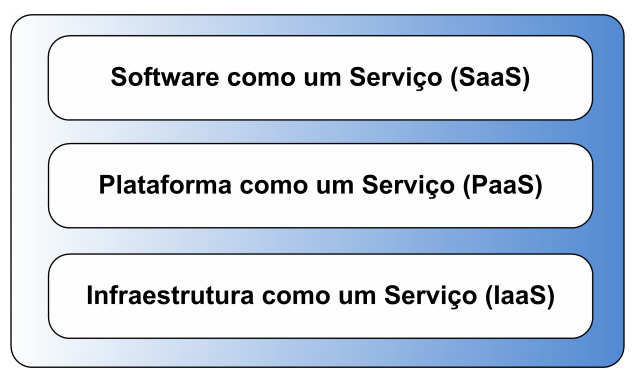
\includegraphics[width=\textwidth]{saas_paas}
		\fonte{\citetexto{Moreira2010}}
	\end{minipage}
\end{figure}
\begin{itemize}
	\item Software como um serviço (Software as a Service - SaaS): Para \citetexto{Mell2012}, é o modelo em que é fornecida ao consumidor a capacidade de utilizar os aplicativos disponibilizados pelo provedor através da Internet. O consumidor não gerencia nem controla a infraestrutura básica, incluindo rede, servidores e sistemas operacionais, nem mesmo as configurações de nenhum aplicativo, tendo a possibilidade de configurar apenas alguns aspectos restritos. Com esse modelo de serviço surge o termo multi-inquilino, no qual os usuários compartilham dos mesmos recursos disponibilizados pelo provedor, porém de forma isolada, ou seja, um não tem conhecimento do outro.
	\item Plataforma como um Serviço (Plataform as a Service - PaaS): Neste modelo de serviço, é fornecido ao usuário a possiblidade de desenvolver e extender aplicações e disponibilizar essas aplicações no serviço de computação em nuvem. O provedor do serviço disponibiliza a infrasestrutura e define uma série de ferramentas, bibliotecas e linguagens suportadas para o usuário. O controle da infrasestrutura é todo gerenciado pelo provedor, ficando o consumidor responsável apenas pela aplicação entregue \cite{Mell2012,verascloud}. Alguns exemplos deste modelo são Amazon Web Services \citetexto{AWS} e SAP Hana Cloud Platform \citetexto{SAPHCP}. 
	\item Infraestrutura como um Serviço (Infraestructure as a Service - IaaS): De acordo com \citetexto{Bhardwaj2010}, é a entrega de capacidade de hardware (rede, armazenamento e servidor), e programas associados (virtualização de sistemas operacionais, sistema de arquivos) como um serviço. Diferentemente do modelo tradicional de hospedagem, é permitido que o usuário aloque os recursos necessários de acordo com a demanda, ao invés de um contrato prévio. O controle que o provedor de IaaS possui é bem menor em comparação ao PaaS, por exemplo. Este se limita a apenas manter o \textit{data center} disponível e operacional o máximo possível. O usuário irá gerir seus softwares e aplicações como se estivesse em sua própria infrasestrutura. Alguns exemplos são Amazon Web Services Elastic Compute Cloud (EC2) e Secure Storage Service (S3) \cite{AWS}.
\end{itemize}
\subsection{Modelos de implantação}
Os modelos de implantação definem como se dará o acesso e diponibilidade da computação em nuvem para o usuário. A diferença entre os modelos se dão de acordo com o tipo de informação e processo de negócio, de acordo com necessidade.  Em alguns casos, por exemplo, não é aceitável para uma empresa ou governo que o \textit{data center} esteja localizado em um outro país. De acordo com \citetexto{Mell2012}, os modelos de implantação podem ser dividos da seguinte maneira:
\begin{itemize}
	\item Nuvem privada (private cloud): A infraestrutura utilizada para computação em nuvem é fornecida exclusivamente para uma única organização, sendo impedido o uso de recursos por qualquer usuário não autorizado pela organização. Neste caso, esta nuvem pode ser administrada por um provedor de serviço em nuvem ou até mesmo pela própria organização.
	\item Nuvem comunidade (community cloud): A infraestrutura é compartilhada por diversas organizações, sendo suportada por uma comunidade com interesses em comum. O gerenciamento dos recursos pode ser feito tanto pelas organizações em questão, quanto por um terceiro (provedor do serviço).
	\item Nuvem pública (public cloud): Este modelo permite que qualquer usuário possa fazer uso dos recursos, desde que conheça a localização do serviço e seja autorizado, normalmente pelo modelo \textit{pay-as-you-go}. Estes modelos são tipicamente oferecidos por grandes organizações que possui uma enorme capacidade de armazenamento e processamento.
	\item Nuvem hibrida (hybrid cloud): Neste modelo, a infraestrutura é composta por dois ou mais modelos de implantação de computação em nuvem (pública, privada, comunitária). Estas infraestruturas são conectadas através de um meio de comunicação, porém, continuando a ser entidades únicas.
\end{itemize}

% TODO: Diferenciar elasticidade e escalabilidade
\section{Elasticidade vs Escalabilidade}
\label{elastic}

A escalabilidade de uma aplicação se diz respeito à quantidade de usuários que ela pode manter conectados ao mesmo tempo, sendo o limite de escalabidade o ponto em que esta não pode suportar mais usuários conectados sem apresentar a mesma  eficiência \cite{Wilder12}. Uma aplicação pode ter a sua escalabilidade estendida através do fornecimento de recursos de \textit{hardware} adicionais, como memória, CPU, largura de banda, etc. No contexto de uma aplicação HPC, uma escalabilidade não se detêm apenas ao número de usuários suportados, mas também ao tipo de processamento que a aplicação precisa executar e que pode precisar de recursos adicionais para continuar desempenhando de forma efetiva. Dessa forma, um sistema é dito escalável quando seu desempenho não se degrada significantemente com o aumento dos usuários ou carga.
Segundo \citetexto{Taurion2012}, elasticidade é a capacidade do ambiente computacional da nuvem aumentar ou diminuir de forma automática os recursos computacionais demandados e provisionados para cada usuário. É a escalabilidade em duas direções: tanto cresce quanto diminui a capacidade ofertada. Os dois termos podem ser confundidos, já que dizem respeito à adaptação de recursos conforme demanda, porém a escalabilidade é relativa à capacidade manter o desempenho conforme a demanda, já a elasticidade é a capacidade de fazer os recursos se adpatem à carga, seja para aumentar ou diminuir. 
Iremos adotar a definição de \citetexto{coutinho2013elasticidade} que diz que a elasticidade é a ``Capacidade de adicionar e remover recursos de forma automática de acordo com a carga de trabalho sem interrupções e utilizando os recursos de forma otimizada.``.

\section{Docker}
\label{docker}

O Docker, apesar de inicialmente utilizar o LXC como provedor de runtime, criou uma implementação própria de ferramenta para criação de containers, procurando resolver algumas limitações da implementação de LXC, como segurança e simplificação [ref].
Alguns dos termos chave para compreender a tecnologia são descritos abaixo \cite{whitepaperDocker2016}:  

\begin{itemize}
	\item Dockerfile - Um arquivo que contém os detalhes de configuração da aplicação, bem como os recursos que esta irá precisar, dizendo ao construtor da imagem como ela deve se parecer.
	\item Docker Image - Este é o resultado do dockerfile, uma imagem que contém um \textit{snapshot} da aplicação. O armazenamento e gerenciamento é feito no \textit{Docker registry}.
	\item Docker Container - A unidade isolada, na qual a aplicação é empacotada, juntamente com todas as bibliotecas e recursos necessários para execução. Em tempo de \textit{runtime} a engine faz a leitura de  uma image e carrega um container.
	\item Docker Engine - A runtime dos containers Docker, com recursos embutidos como: orquestração de containers, rede  e segurança que é instalado no host, seja virtual (VM) ou cloud (AWS, Azure, Google Cloud Enterprise etc).
	\item Docker Registry - Um serviço no qual são armazenadas as imagens Docker, além de serem protegidas e gerenciadas. No Docker registry é possível armazenar múltiplas versões de uma imagem (aplicação), através do uso de \textit{tags}. Com isto, é possível fazer uma atualização de uma imagem facilmente, através de uma modificação na imagem e armazená-la com uma versão diferente, sem comprometer a versão estável.
\end{itemize} 

\subsection{Containers}

A palavra \textit{container} ficou popularizada a partir de uma técnica de isolamento de recursos dentro de um sistema operacional baseado em UNIX, desde a release do sistema operacional Solaris 10 em 2005. A ideia era não somente restringir o acesso de recursos dentro deste container, mas também permitir uma proteção de recursos explicitamente dedicados à estes containers. Embora seja considerada como uma \textit{best practice} em desenvolvimento, a utilização de containers é bastante complexa e o mal uso pode levar à criação de aplicações com brechas de segurança, embora se pressuponha o contrário, diferente da facilidade que se tem com a utilização de máquinas virtuais (VM). Uma das implementações atuais de containers é o Linux Containers (LXC), que provê uma série de ferramentas que trabalham nativamente em sistemas operacionais baseado em UNIX para fornecer um ambiente semelhante ao que se obtêm com VM's, mas sem a sobrecarga de rodar um kernel separado e fazer simulação de hardware, através de utilização de namespaces, e \textit{control groups} \cite{LXC2016}.
Recentemente, a utilização de containers se popularizou em meio ao desenvolvimento de computação para a nuvem por causa da nova ferramenta chamada \textit{Docker}, criada em 2013 e inicialmente baseada no LXC como um provedor de runtime. Segundo \cite{NICKOLOFF2016}, Docker é um conjunto de ferramentas e serviço que facilitam a criação e manipulação de containers dentro de um sistema baseado em UNIX. Com Docker, é possível ter todas as vantagens de utilização de containers, porém sem o alto custo de configuração e com containers fornecidos seguindo as melhores práticas. 

\subsection{cgroups}
Cgroups é uma configuração que faz parte do subsistema de kernel de sistemas baseado em UNIX, que fornece controle sobre recursos do sistema, como CPU, memória, rede, etc. O cgroups, ou control groups esta presente na implementação de containers de Docker e é utilizado como mecanismo base de gerenciamemnto de recursos \cite{NICKOLOFF2016}.

\subsection{chroot}
Chroot (\textit{change root}) é um comando Linux para mudar o diretório root do processo corrente e seus processos aninhados para um novo diretório. Alguns containers utilizam este comando para isolar e compartilhar o sistema de arquivos entre os ambientes containerizados \cite{Dua2014}. 

\section{Virtualização vs Containerização}
\label{virtualization}

Uma camada de virtualização pode ajudar a isolar um ambiente compartilhado de computadores. Em clusters de HPC, normalmente os recursos são compartilhados entre mais usuários e isto faz com que possa ocorrer problemas nesse compartilhamento \cite{Xavier2013}.
A camada de virtualização baseada em container possui uma performance muito superior à virtualização pura, segundo a pesquisa deles.


% Substituir o uso de VM no autoelastic e fazer testes de viabilidade de containers no lugar
% verificar vantagens e novas oportunidades que o autoelastic pode ter com containers.
% Fazer um comparativo - Docker vale a pena?
% Talvez modificar o formato de balanceamento de carga, já que containers podem ter menor custo.

\subsection{Virtualização baseada em Hypervisor}
Um \textit{hypervisor}, ou gerenciador de máquinas virtuais, é um programa que roda no sistema operacional host, fornecendo os recursos de hardware deste para uma série de máquinas virtuais, neste caso, estas máquinas virtuais compartilham o mesmo hardware. Como mostrado na figura~\ref{fig:vmvsdocker}, o hypervisor é responsável por fornecer o acesso aos recursos para cada sistema operacional dentro das máquinas virtuais, mas com o custo deste gerenciamento como processamento, já que a ferramenta procura fornecer comportamento fiel de hardware para as máquinas virtuais \cite{Zhang2016}.

\subsection{Virtualização baseada em container}

O termo \textit{containerização} é a forma popular para se referenciar à virtualização baseada em container, que permite o isolamento de determinados softwares, que são executados dentro do mesmo kernel no sistema operacional Linux, mas que diferentemente do hypervisor, não adiciona uma camada virtualização, na qual precisaria carregar um sistema operacional convidado \cite{Zhang2016}, como mostra a figura~\ref{fig:vmvsdocker}.
\cite{Dua2014}

A Figura~\ref{fig:vmvsdocker} ilustra a diferença entre uma aplicação em uma camada de virtualização por Docker e VM.

\begin{figure}
	\caption{Docker vs Virtual Machine}
	\label{fig:vmvsdocker}
	\centering%
	\begin{minipage}{.4\textwidth}
		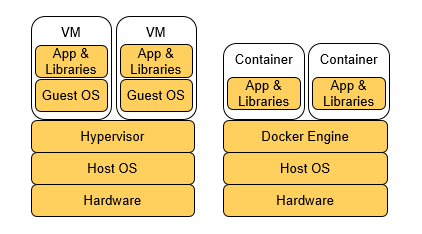
\includegraphics[width=\textwidth]{vmvsdocker}
		\fonte{\citetexto{Cham12}}
	\end{minipage}
\end{figure}

\begin{table}[!ht]
	\caption{Características de VM e Containers}
	\label{tab:table1}
	\centering
	\resizebox{\textwidth}{!}{%
		\begin{tabular}{|l|l|l|}
			\hline
			\textbf{Parametro} &\textbf{Máquinas Virtuais}\ &\textbf{Containers}\\
			\hline
			SO Convidado & \begin{tabular}[c]{@{}l@{}}Um hardware virtual é disponibilizado para cada VM, \\ com um espaço de memória reservado.\end{tabular} & \begin{tabular}[c]{@{}l@{}}Todos os convidados compartilham o mesmo SO,\\cada imagem é carregada para o espaço de memória \\do Kernel \end{tabular}\\ \hline
			Comunicação & Feita por dispositivos Ethernet & Utilização de mecanismos IPC como sinais, sockets, pipes\\ \hline
			Segurança & Depende da implementação do fornecedor de Hypervisor & Utilização de mecanismos de controle de acesso\\ \hline
			Desempenho & \begin{tabular}[c]{@{}l@{}}Irá receber uma sobrecarga pelo trabalho de tradução\\de instruções do sistema hospedeiro para o convidado\end{tabular}  &\begin{tabular}[c]{@{}l@{}}Containers fornecem um desempenho muito próximo ao \\nativo em comparação ao executado direto no hospedeiro\end{tabular} \\ \hline
			Isolamento &\begin{tabular}[c]{@{}l@{}} Não é possível compartilhar arquivos, bibliotecas e \\execução de programas entre as máquinas virtuais  \end{tabular} & \begin{tabular}[c]{@{}l@{}}Subdiretórios podem ser montados e compartilhados \\ entre containers no mesmo hospedeiro \end{tabular} \\ \hline
			Tempo de início & \begin{tabular}[c]{@{}l@{}} Demora o tempo de processo de boot de um \\ sistema operacional \end{tabular} & Containers não fazem boot de sistema\\ \hline
			Armazenamento & \begin{tabular}[c]{@{}l@{}}Software específicos de armazenamento e sistema \\de arquivos precisam ser instalados no convidado \\além de estarem no hospedeiro\end{tabular} & \begin{tabular}[c]{@{}l@{}} O armazenamento em containers pode ser \\ compartilhado com o hospedeiro \end{tabular} \\ 
			\hline
		\end{tabular}}
		\fonte{\cite{Dua2014}}
\end{table}

\chapter{Trabalhos Relacionados}
\label{related}
Neste capítulo iremos ver um estudo de diversos trabalhos, os quais trazem soluções para elasticidade para aplicações de alto desempenho, bem como estudos comparativos entre a utilização de máquinas virtuais e containers. Serão apresentados os detalhes cada trabalho no início, e ao término do capítulo será feito uma comparação entre as abordagens.

\section{Seleção de Trabalhos}

A seleção de trabalhos relacionados, bem como outras referências para esta monografia, foi realizada através de uma pesquisa em diversas bases de dados de artigos científicos de Ciências Exatas, como o site da IEEE, ACM Digital Library e Springer Link. Também foram consultadas bases de dados nacionais, como o Portal de Periódicos CAPES/MEC e também a base de dados Biblioteca Unisinos. 
Para a realização das pesquisas nessas diversas bases de dados, foram utilizadas buscas com estas principais palavras-chave: \textit{docker virtual machine, container high performance computing, scalablity elasticity, hpc application container, virtualization containers, cloud computing elasticity}. O resultado dessas pesquisas foi analisado com o intuito de encontrar trabalhos que explorassem a utilização de containers em ambientes de cloud computing, bem como as alternativas e implementações de elasticidade em aplicações HPC. Na sessão \ref{autoelastic} foi selecionado um trabalho que implementa um modelo de elasticidade para aplicações HPC, fornecendo recursos para a aplicação de forma dinâmica, através de provisionamente de máquinas virtuais em nodos de computação, conforme a demanda da aplicação \cite{7090978}. Nas sessões subsequentes, (\ref{trabdocker}) foram selecionados trabalhos que utilizam containers para implementação de ambientes de HPC e que traçam um comparativo da utilização de máquinas virtuais e containers. 
Por fim, na sessão \ref{comparison}, é realizado um comparativo dos trabalhos encontrados, bem como uma conclusão acerca das possibilidades, tendo em vista a análise do modelo já implementado, o AutoElastic, e as lacunas encontradas.

\section{AutoElastic}
\label{autoelastic}

Segundo a definição de \citetext{Facco2016} para a ferramenta AutoElastic:
\begin{quote}
AutoElastic age como um \textit{middleware} permitindo que aplicações HPC iterativas obtenham vantagem do provisionamento de recursos dinâmico de uma infraestrutura de nuvem sem a necessidade de modificações no código fonte. AutoElastic oferece a elasticidade de forma automática, não sendo necessária a configuração de regras por parte do usuário.
\end{quote} 
O problema apresentado pelo trabalho é que muitas das abordagens atuais do mercado, para fornecer elasticidade em aplicações HPC, necessitam de uma intervenção do usuário para fazer tais configurações de elasticidade, ou seja, definir o momento em que serão adicionados ou removidos recursos, através de manipulação de máquinas virtuals, disponíveis para a aplicação, seja por uma configuração estática de \textit{threshold} ou de uma configuração no código da aplicação. O desenvolvimento do \textit{middleware} AutoElastic permite um modelo transparente ao usuário em questão de configuração de parâmetros. O AutoElastic possui um protótipo executado pelo autor na plataforma de nuvem OpenNebula e obteve resultados de ganho de desempenho de até 59\% na execução de uma aplicação de integração numérica \textit{CPU-Bound}, quando comparada com outras soluções de elasticidade. 

\section{Utilizando Docker para Aplicações de Alto Desempenho}
Neste estudo, \citetext{7562612} faz um estudo comparativo de máquinas virtuais e containers, além de propor um modelo de \textit{deploy} de aplicações distribuídas em Docker containers. Para verificar o modelo proposto, foram realizados testes utilizando duas aplicações HPC que requerem grande capacidade computacional, Graph500 e Linpack (HPL). Para manter um base de comparação, foram realizados execuções com processamento nativo, sem adição de camada de virtualização. Os testes executados mediam os custos computacionais dos processos, considerando diversas combinações de instâncias de máquinas virtuais e instâncias de containers, sem levar em consideração a elasticidade. Na conclusão do trabalho, foi notado que Docker containers possuem um desempenho mais eficiente para processamento massivo de dados do que máquinas virtuais, que por sua vez, possuem uma implementação de isolamento mais confiável. 

\section{Virtualization vs Containerization to support PaaS}
% O texto possui uma tabela de comparação das tecnologias, bem como de relação de PaaS com containers.
% Não se aprofunda muito na questão de comparação, mas pode ser extendido.
\cite{Dua2014} Apresenta um estudo sobre como provedores de PaaS estão utilizando containers para encapsular aplicações. O estudo endaga a atual adoção de plataformas baseadas em containers e explora diversas implementações de containers, entre elas: Linux Containers, Docker, Warden Container, lmctfy e OpenVZ. A análise foi feita baesada em como cada uma das tecnologias lidam com processos, sistema de arquivos e isolamento de namespaces, dando uma atenção especial à características únicas de cada implementação. Por fim, o trabalho busca fazer uma análise dos fatores que afetam a adoção de containers e possíveis funcionalidades que estão em falta para uma nova geração de PaaS.

De acordo com os autores, containers possuem uma vantagem inerente sobre máquinas virtuais, devido à melhorias de performance e redução de tempo de \textit{start up}. Apesar de existirem diversas soluções de containers no mercado, cada uma com prós e contras, eles tendem a manter um padrão, principalmente em relação ao uso de \textit{chroot} e \textit{namespaces}. Ressalta-se que Docker aplica camadas adicionais em cima da solução nativa Linux Containers, tornando a solução muito mais interoperável e mais interessante para provedores que não querem ficar presos à arquiteturas específicas. Já a solução OpenVZ se mostrou melhor em termos de segurança, porém isto associado ao custo de se ter um kernel customizado para a aplicação.

\section{Performance Evaluation of Container-based Virtualization for High Performance Computing Environments}
% Este estudo possui gráficos de comparação, porém o container está no nível IaaS, um pouco diferente do que preciso.
\cite{Xavier2013} Inicia o seu estudo abordando a utilização de tecnologias de virtualização para aplicações de alto desempenho, alegando que tais tecnologias foram tradicionalmente evitadas ao longo dos anos por sua adição de camadas que comprometem desempenho, o que é crucial para tais aplicações. Porém, como o advento de implementações de virtualização baseada em containers, o autor indaga que é possível se obter uma sobrecarga muito pequena com a utilização de tecnologias como Linux VServer, OpenVZ e Linux Containers (LXC), chegando a um desempenho quase nativo. Para embasar o questionamento, foi feito um comparativo de desempenho utilizando tais tecnologias e um modelo tradicional de virtualização, o Xen. 

Os experimentos feitos pelo autor utilizaram programas de avaliação de desempenho de supercomputadores fornecidos pela NASA \cite{NASA2016}. Os programas executados possuem diferentes focos de estressamento da aplicação, permitindo identificar o compartamento das implementações sob os mais diversos cenários. A partir da análise, se viu que os sistemas baseado em containers possuem uma performance muito próxima da nativa, tanto para CPU, memória, disco e rede, ficando a principal diferença na implementação de gerenciamento de recursos, no caso de  LXC, por exemplo, isolamento e segurança é garantido apenas por uso de \textit{cgroups}. O estudo critica o desempenho das implementações para isolamento de memória, disco e rede, mas considera um sucesso o isolamento de CPU. Apesar do provisionamento de recursos não estar completamente maduro para estas soluções, é importante perceber que para aplicações de alto desempenho, muitas vezes a CPU é o mais importante, além disto, essas aplicações normalmente não exigem a alocação compartilhada de partição do cluster para multiplos usuários ao mesmo tempo. Por fim, a implementação LXC foi considerada a melhor alternativa para substituir o modelo tradicional de virtualização em apliações HPC, se for considerado apenas o quesito CPU, no comparativo, a implementação obteve um desempenho muito próximo ao nativo, ou seja, o container executou os programas de teste com praticamente o mesmo potencial que a própria máquina, enquanto a implementação utilizando máquina virtual (XEN) obteve uma sobrecarga de aproximadamente 4.3\%.

\section{Performance Characterization of Hypervisor and Container-based Virtualization for HPC on SR-IOV Enabled InfiniBand Clusters}

Neste trabalho, \citetext{Zhang2016} fazem uma análise das vantagens de se utilizar virtualização em ambientes, como independência de hardware, isolamento e fácil gerenciamento, através de tecnologias de \textit{hypervisor}, como Xen, KVM e VMWare, mostrando que sua utilização hoje, é fundamental para o desenvolmento de computação em nuvem. Especificamente, se aborda a sobrecarga que tais soluções possuem em relação aos dispositivos de I/O virtualizados.

A utilização de passagem PCI (\textit{Peripheral Component Interconnec}) fornece os meios para dar uso exclusivo de recursos para dispositivos de I/O, como controlador de disco, rede, placa de vídeo, etc, dando um melhor desempenho para a máquina virtual. Em contrapartida, isto impede o uso compartilhado entre diversas máquinas virtuais de determinado recurso. O trabalho apresenta SRV-IOV (\textit{Single Root I/O Virtualization }) para permitir o compartilhamento entre conexões de alto desempenho, como InfiniBand, além de introduzir testes utilizando containers ao invés de máquinas virtuais, buscando atingir um desempenho mais próximo do nativo.

Em resumo dos testes executados, utizando aplicações de \textit{benchmark} com MPI, as avaliações identificaram que VM com passagem PCI é mais eficiente que VM com SR-IOV habilitado, entretanto a solução é a maneira mais eficiente de se poder compartilhar recursos de I/O. No geral, soluções baseadas em containers conseguem entregar com mais desempenho que modelos baseados em hypervisor. Em comparação ao desempenho nativo, os testes identificaram uma sobrecarga de no máximo 9\% para aplicações HPC.

\section{Is Container-Based Technology a Winner for High Performance Scientific Applications?}
\citetext{Adufu2015} Conduziu testes para demonstrar que, durante a execução de aplicações científicas em ambientes HPC, o tempo médio de processamento em um sistema com virtualização baseada em containers é menor do que o tempo em um sistema baseado em \textit{hypervisor}, isto devido ao tempo de \textit{start-up}. Para gerar os resultados de comparação, foi utilizado a ferramenta \textit{autodock3}, um programa de simulação de modelagem molecular. Para gerenciar os containers, a ferramenta Docker foi utilizada, mostrando um gerenciamento de recursos mais eficiente, até mesmo no cenário em que foi alocado mais memória do que realmente disponível fisicamente para as instâncias em execução. 
O trabalho conduzido indicou que sistemas baseados em containers são mais eficientes que sistemas baseados em máquinas virtuais, além de possuir um gerenciamento de memória mais eficiente entre as aplicações executadas em paralelo, o que o torna uma solução mais atrativa para o desenvolvimento de ambientes para aplicações HPC.

\section{Comparativo dos trabalhos relacionados}
Nesta sessão, irei mostrar esta tabela.

\begin{table}[]
\centering
\caption{My caption}
\label{my-label}
\resizebox{\textwidth}{!}{%
\begin{tabular}{|l|l|l|l|l|l|l|}
\hline
\textbf{Trabalho} & \textbf{Tecnologia}  & \textbf{Elasticidade} & \textbf{Base de Comparação}     & \textbf{Métricas}                                                                   & \textbf{Plataforma}  & \textbf{Testes}                                                              \\ \hline
\cite{Facco2016}       & VM                   & Sim                   & \begin{tabular}[c]{@{}l@{}}nodo puramente alocado\\(nativo) \end{tabular}  & desempenho, custo e energia                                                         & OpenNebula           & cálculo de integrais                                                         \\ \hline
\cite{7562612}                 & Docker               & Não                   & CentOS 7 64-bit 3.10.0          & Performance por instancias                                                          & OpenStack            & \begin{tabular}[c]{@{}l@{}} MPI com Graph500,\\ Linpack\end{tabular}                                                   \\ \hline
\cite{Xavier2013}                 & \begin{tabular}[c]{@{}l@{}} LXC, OpenVZ,\\ VServer \end{tabular} & Não                   & Ubuntu 10.04 LTS                & \begin{tabular}[c]{@{}l@{}}diversos tipos de \\ recursos em único nodo\end{tabular} & 4 computadores fixos & \begin{tabular}[c]{@{}l@{}}Linpack, STREAM, \\ IOZone, NetPIPE\end{tabular} \\ \hline
\cite{Zhang2016}                 & Docker               & Não                   & CentOS Linux                    & \begin{tabular}[c]{@{}l@{}}desempenho de operações\\ de comunicação\end{tabular}    & OpenStack            & \begin{tabular}[c]{@{}l@{}}MPI com Graph500,\\ NAS, LAMMPS\end{tabular}     \\ \hline
\cite{Adufu2015}                 & Docker               & Não                   & Ubuntu 14.04 Trusty Tahr        & \begin{tabular}[c]{@{}l@{}}Desempenho de memória \\ RAM\end{tabular}                & OpenStack            & \textit{autodock3}                                                                    \\ \hline
\end{tabular}}
\end{table}

Trabalho - tecnologia - operações - base de comparação - métricas - plataforma - tipo de teste 
AutoElastic \cite{Facco2016} - VM - elasticidade por alocação - nodo puramente alocado (nativo) - desempenho, custo e energia - OpenNebula - cálculo de integrais.
Using Docker in high performance computing applications \cite{7562612} - Docker containers, sem elasticidade, CentOS 7 64-bit 3.10.0, performance por instancias, OpenStack, MPI com Graph500 e Linpack.
Performance Evaluation of Container-based Virtualization for High Performance Computing Environments \cite{Xavier2013} - LXC, OpenVZ, VServer,  - sem escalabilidade - Ubuntu 10.04 LTS - diversos tipos de recursos em único nodo - 4 computadores fixos -Linpack, STREAM, IOZone, NetPIPE.
HPC on SR-IOV Enabled InfiniBand Clusters \cite{Zhang2016} - Docker - sem elasticidade - CentOS Linux - desempenho de operações de comunicação - Chameleon Cloud (OpenStack) - MPI com Graph500, NAS, LAMMPS.
Is Container-Based Technology a Winner for High Performance Scientific Applications? \cite{Adufu2015} - Docker - sem escalabilidade - Ubuntu 14.04 Trusty Tahr - Desempenho de memória RAM - OpenStack - autodock3


%Melhorar
Concluo que o aproveitamento máximo de recursos, utilizando uma camada de virtualização de fácil implementação e não muito dependente do sistema operacional é objetivo de um ambiente próprio para execução de aplicações de alto desempenho. Portanto, os trabalhos analisados deixaram uma lacuna em relação a esta questão por não apresentarem uma solução que utilize uma tecnologia mais eficiente para processamento do que máquinas virtuais para alocação de recursos em aplicações de alto desempenho. Alguns trabalhos abordaram o uso de containers para aplicações de alto desempenho, porém apenas executando programas de testes para comprovar a possibilidade de uso, sem aplicar em infraestrutura que possa fornecer os recursos para as aplicações. O objetivo do trabalho que traz o AutoElastic de \citetexto{Facco2016}, juntamente com a possibilidade de se otimizar a utilização de recursos utilizando containers é o que justificou a abordagem tomada por este presente trabalho.

%=======================================================================
% Modelo
%=======================================================================
\chapter{Modelo}
\label{model}

\section{Questões de projeto}
Objetivo deste trabalho é propor uma melhoria para o modelo de elasticidade em nuvem para aplicações HPC iterativas (AutoElastic). A partir da substituição do componente de criação de recursos com a criação de máquinas virtuais por containers, espera-se atingir uma melhoria no tempo de espera para se ter os recursos computacionais disponíveis após a requisição. Com os resultados, será analisado em que situações os containers tem um desempenho melhor, podendo propor uma abordagem diferente de ação quando se atinge os \textit{thresholds}, fazendo o melhor uso da tecnologia. Portanto, o modelo proposto tem como escopo somente trabalhar nos recursos computacionais fornecidos para o modelo AutoElastic. 

%TODO
Desenvolver um modelo de elasticidade automática adaptada para uso de containers, para aplicações de Computação de Alto Desempenho, em ambientes de computação em nuvem, com foco em otimizar a utilização de recursos, em comparação ao método de elasticidade automática baseado em virtualização de máquinas.

No início deste trabalho propusemos a seguinte questão de pesquisa: Como seria o modelo de elasticidade em nuvem adaptado para o uso de containers para aplicações HPC iterativas, que possa gerar um ganho significativo de economia de recursos? Sabemos, até o ponto deste estudo, que é possível sim ter um ambiente virtualizado utilizando containers, que pode substituir um ambiente com virtualização baseada em \textit{hypervisor}. Mas para responder a pergunta por completo, ou seja, identificar o ganho de economia de recursos e de desempenho, é necessário fazer ajustes baseados no desempenho do modelo após a substituição do componente, sempre se preocupando em que se permita utilizá-lo em tempo de execução sem um aumento acentuado de overhead.

Para que se possa manter o foco no real propósito deste trabalho, partiremos do modelo atual do AutoElastic, que já possui uma implementação definida como protótipo. Sendo assim, como resultado deste modelo não teremos uma implementação genérica ou adaptável, ou ao menos esta não será uma preocupação de projeto, visto que os objetivos principais são o ganho de desempenho em comparação ao modelo atual, a substituição do componente de virtualização será feita utilizando as mesmas tecnologias empregadas. 

Não será criada uma API detalhada neste momento. E até mesmo os resultados da comparação não receberão um tratamento para serem consumidos por uma ou outra plataforma específica. Pois entendemos que estas são questões secundárias, e não influenciam no propósito principal do trabalho. Optando assim por manter baixa a complexidade do projeto. E de igual forma, usaremos uma plataforma de cloud arbitrária que julgarmos mais apropriada para a execução dos testes com o modelo, sem preocupação com compatibilidade com outras pelos mesmos motivos já descritos nesta seção.

\section{Arquitetura}

TODO

\section{Metodologia de Avaliação}
TODO



%=======================================================================
% CONCLUSÃO
%=======================================================================
\chapter{Conclusão}
\label{conclusion}

TBD
\section{Cronograma}
Abaixo encontramos uma tabela com a relação de atividades previstas para o desenvolvimento deste trabalho, com um planejamento das suas respectivas datas de execução.

\begin{tabular}{|l|c|c|c|c|c|c|}\hline
 & \multicolumn{6}{c|}{\textbf{Meses}}\\ \cline{2-7}
\raisebox{1.5ex}{\textbf{Etapa}} & 01 & 02 & 03 & 04 & 05 & 06 										\\ \hline

Estudo e escolha da plataforma de cloud computing 						& X &   &   &   &   &		  	\\ \hline
Estudo e preparação do ambiente de execução de testes            		& X &   &   &   &   & 			\\ \hline
Modelagem da solução			 										& X & X &   &   &   &			\\ \hline
Definir estratégia para comparação de resultados						&   & X &   &   &   & 			\\ \hline
Desenvolvimento da extensão de balanceamento de carga					& 	& X &	&   &   &			\\ \hline
Testes e avaliação do balanceamento de carga							& 	& X & 	& 	& 	&  		   \\ \hline
Escrita do artigo														& X	& X & X & X & X & X			\\ \hline
Preparação da apresentação												& 	&   &   &   & X & X			\\ \hline
Baterias de testes para validação 										& 	& 	& 	& 	& 	& X 	   \\ \hline
Avaliação e tratamento dos resultados									& 	& 	& 	& 	& 	& X 	   \\ \hline

\end{tabular} 

\label{t_cronograma}

%=======================================================================
% Referências
%=======================================================================
\bibliography{exemplo}

%=======================================================================
% Exemplo de Apêndice
% O Apêndice é utilizado para apresentar material complementar elaborado
% pelo próprio autor.  Deve seguir as mesmas regras de formatação do
% corpo principal do documento.
%=======================================================================
\appendix
\chapter{Informações Complementares}

O Apêndice é o lugar para incluir textos complementares, que não são essenciais para o entendimento do assunto principal da monografia, mas que podem contribuir com informação relevante (por exemplo, uma prova matemática, uma conceituação básica, etc.).  Ele deve seguir o formato normal do documento.

%=======================================================================
% Exemplo de Anexo
% O Anexo é utilizado para a ``inclusão de materiais não elaborados pelo
% próprio autor, como cópias de artigos, manuais, folders, balancetes, etc.
% e não precisam estar em conformidade com o modelo''.
%=======================================================================
\annex
\chapter{Artigos Publicados}
Existe diferença entre os Apêndices e os Anexos.  Os apêndices trazem informação escrita pelo próprio autor do trabalho, incorporando-se ao formato da monografia como um todo.  Já um anexo é um material à parte, definido/publicado por si só, e que o autor julga conveniente ser apresentado juntamente com a monografia.  Normalmente também vai apresentar formato próprio, como um artigo publicado, um folder, uma planilha, etc.
\end{document}
